\chapter{Conclusion and Discussion}
\section{Conclusion}
\setlength{\parindent}{2.5em}
This project presents a helmet and head detection system developed using a custom-trained YOLOv8 model, integrated with a counting mechanism applied to university CCTV footage for real-world evaluation. The final model demonstrated significant improvements in detection accuracy, achieving up to 95\% accuracy in helmet detection and an average of 91.75\% across all object classes in the test videos. 

The implementation of the double-line counting method proved effective in reducing duplicate counts and stabilizing detection outputs, particularly for slow-moving or partially occluded objects. For person and motorbike tracking, the BoT-SORT tracking algorithm delivered reliable performance under low-overlap conditions, supporting accurate and consistent count results. Challenges in person detection—such as undetected children and overlapping riders—were addressed by aggregating helmet and head detections to approximate the total number of individuals, a decision supported by the high precision of the helmet and head models. Additionally, flickering and inconsistent detections in motorbike tracking were mitigated through the use of tracker history, which preserved object IDs across frames and allowed for movement-based counting based on bounding box center positions. This approach enhanced stability and reduced false counts. A defined Region of Interest (ROI) was also applied to ensure that only relevant objects within the designated monitoring area were included in the count, avoiding erroneous detections from peripheral motion. Overall, the system demonstrates strong potential for practical applications in automated helmet usage monitoring and traffic safety analytics.

To effectively use this helmet and head detection and counting system, several key components and considerations should be followed. The core of the system is a custom-trained YOLOv8 model, which achieved high detection accuracy across all classes, with helmet detection reaching up to 95\% and an overall average accuracy of 91.75\%. For counting, the system employs two methods: a double-line counting mechanism for helmets and heads, which effectively reduces duplicate counts in cases of slow movement or occlusion, and the BoT-SORT tracking algorithm for person and motorbike counting, which improves consistency by tracking object IDs across frames. In scenarios where person detection is unreliable—such as detecting children or overlapping riders—the counts of helmet and head detections are combined to estimate the number of persons, leveraging the accuracy of the custom-trained models. To handle flickering or missed detections, the system uses the track history feature of the tracker, which compares the current position of an object with its previous location to ensure continuity in tracking. Additionally, a Region of Interest (ROI) should be defined to limit the detection and counting zone, preventing errors caused by objects entering or leaving the frame. This system is most effective when applied to CCTV footage in controlled environments with stable camera positions and clearly defined detection areas.



\section{Discussion}
\subsection{Model Improvement}
\setlength{\parindent}{2.5em}
Table 4.1 highlights the performance improvement of various helmet detection models, while person and motorbike detection accuracies remain constant across all models at 87\% and 96\%, respectively. This consistency is expected, as all models use the original YOLOv8 architecture for detecting persons and motorbikes. The main focus of model optimization lies in helmet detection, which has undergone several iterations of training using custom datasets. The earliest version, BestV8, achieved only 42\% accuracy in helmet detection, likely due to limited training data or suboptimal labeling. This was significantly improved in Best21, which reached 72\% accuracy. Subsequent models, such as Helmet\_model and Head\_model, showed further improvements to 82\% and 86\%, respectively, indicating better dataset quality and fine-tuning strategies. The most refined version, Best17, achieved a 95\% helmet detection rate, demonstrating the effectiveness of progressive model training, class balancing, and more consistent annotation.
\subsection{Helmet and Head Double Line Counting}
\setlength{\parindent}{2.5em}  % or however much indent you want
In the first video which is table 4.2, the accuracy of our helmet and head detection are very precise, since the video displays a clear bounding box of head and helmet detection and no overlapping with other head and helmet. Table 4.2 showing the accuracy of non-helmet to be at 100\%, but there are minor flaws in helmet accuracy as it exceed the ground truth. The reason there are 26 helmets being displayed from the counting system is because the person who is in the front often blocks out the person who is in the back and this can cause false detection, classifying people who are not wearing a helmet as wearing it.

In the second video which is table 4.3, the accuracy went down compared to the first video. The reason is that there are many occasions where multiple motorbikes come through at the same time, causing confusion of our model and causing many overlapping bounding boxes of head and helmet. This makes the accuracy of helmet detection to 82\% and non-helmet to 90\%.

\subsection{Person and Motorbike BotSort Counting}
\setlength{\parindent}{2.5em}  
Table 4.4 shows the accuracy of person detection to be 98\% and motorbike accuracy to be 93\%. this result is being tested on video 1, which is the video where overlapping hardly appear, making the result satisfying.


Table 4.5 which is being tested on the second video where this video overlapping appears often more than the first video resulting in lower accuracy comparing to the first video. As person accuracy drop down to 93\% and motorbike drop to 77\%. Occasionally motorbike with two person on it can cause confusion in bounding boxes and it can appear to detect one person instead of two person, since the people who is driving and riding is really close to each other. Our BotSort method works well with less overlapping of bounding boxes, and as the more over-lapping occur, it causes a confusion of unique ID tracking system when it is in the counting zone. Causing a new unique ID to be create eventhough it is consider the same person or motorbike proceeding throughout the frame. 



\section{Limitation}

\begin{center}
	\begin{minipage}{0.45\textwidth}
		\centering
		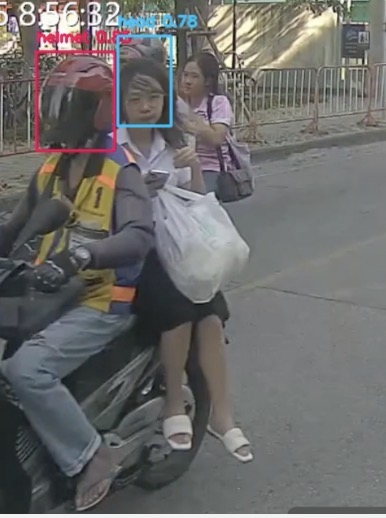
\includegraphics[width=\linewidth]{limitation2.png}
		\vspace{0.5em} % Adjust as needed
		
		\textbf{Figure 5.1}
	\end{minipage}
	\hfill
	\begin{minipage}{0.45\textwidth}
		\centering
		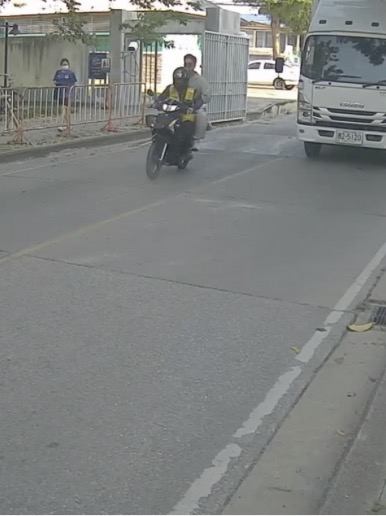
\includegraphics[width=\linewidth]{limitation3.png}
		\vspace{0.5em} % Match the first one
		
		\textbf{Figure 5.2}
	\end{minipage}
\end{center}
\setlength{\parindent}{2.5em}
During system development and testing, the main challenge involved dealing with overlapping bounding boxes, particularly when multiple motorcycles and riders appeared close together. This sometimes led to incorrect object counts or detection errors, such as merging two people into one or misidentifying a detection. The tracking system also struggled when many objects entered the counting zone at once, occasionally creating new IDs for the same object however we uses Bot\_sort Tracker to help minimize the flickering as possible, as when they enter the counting zone, if object is redetected there are chances new ID will appear and our system could not reidentify the object, it would count that object base on the new ID.

 These issues were more pronounced in crowded scenes and highlight the limitations of relying on bounding box-based tracking in complex real-world environments. which can be seen in Figure 5.1. This sometimes led to incorrect object counts or detection errors, because there are another object blocking another object in the counting zone. 

In Figure 5.2 another flaw showing the struggle of tracking system when an object appear to be on another lane, causing it hard for our model to detect an object, especially when it appear to far from the annotation point.


\section{Future Work}
\setlength{\parindent}{2.5em}
In future improvement, the focus will be on improving both the detection model and the tracking accuracy. Training with more diverse and balanced data will help the model generalize better across various environments and video conditions. Further enhancement of the counting and tracking logic is also planned to address issues with ID switching and occlusion. Additionally, while deployment to the university server is not yet complete, it remains a key objective for real-time monitoring in a practical setting. These improvements will support the goal of developing a more accurate, stable, and scalable helmet compliance monitoring system.



